\documentclass[12pt,twocolumn]{article}
	\usepackage[portuguese]{babel}
	\usepackage[utf8]{inputenc}
	\usepackage[T1]{fontenc}
	
	\usepackage[legalpaper, left=8mm, right=8mm, top=2cm, bottom=2cm]{geometry}	
%	\usepackage{multicol}
	
%	\usepackage{lipsum}
	\usepackage{amsmath}
	
	
	
%	\usepackage{wrapfig} 
	\usepackage{graphicx}
	\graphicspath{{./fig/}}
	
	\newcommand{\msg}[1]{\textsf{\textit{#1}}}
	\renewcommand{\thefigure}{\thesubsection\alph{figure}}

%opening
\title{Multicast Confiável}
\author{Guilherme Akira Demenech Mori}

\begin{document}	
	
	%\sffamily 
	
	%\begin{multicols}{2}		
		
		\maketitle	
	
		\begin{abstract}
			
			Este trabalho descreve o problema, a proposta e o programa de multicast confiável.
			Com base nas restrições de comunicação ponto-a-ponto, detecção de e tolerância a falhas e de aumento de escala, são apresentados dois protocolos para envio de mensagens de um host para muitos sem utilização de broadcast.
			No final, é detalhada a implementação e seu uso.
		\end{abstract}
	
		\tableofcontents
		
		\listoffigures
	
	%\end{multicols}

	%\begin{multicols}{3}
	
		\section*{Contextualização}
			Comunicação é um aspecto essencial da vida humana na Terra.
			Seres humanos, assim como vários outros animais sociais, dependem das relações com outros indivíduos.
			Vemos essa dependência, material e psicológica, se expressar nos mais diversos contextos: divisão do trabalho, amizade, afetividade etc.  
			
			O desenvolvimento da linguagem demonstra a importância da comunicação para a sociedade.
			De fato, é difícil imaginar a organização social sem alguma padronização de comunicação.
			Os protocolos de telecomunicação criam padrões muito mais restritivos que a linguagem natural (isto é, os idiomas humanos) e permitem transmissão de dados por longas distâncias entre dispositivos de inúmeros fabricantes.						  
	
			\subsection{Definição do problema}
				Utilizando somente comunicação ponto-a-ponto, propor protocolos que garantam a entrega a múltiplos hosts ou que detectem quais apresentaram falhas.  		
				Deve-se buscar reduzir o tráfego da rede como um todo e também a sobrecarga de hosts individuais.
				
				O host remetente deve identificar quais destinatários confirmaram recebimento e qual foi o intervalo de tempo para detectar falha. 
				Da mesma forma, os hosts destinatários devem exibir a mensagem recebida somente uma vez, confirmando recebimento.
				
				Os hosts poderão ser identificados por nomes, para facilitar a diferenciação entre eles e para auxiliar o(a) usuário(a) humano(a) a memorizá-los.							
						
		\section{Unicast}
		
			Para se enviar uma mensagem para somente um destinatário, basta que o host envie e aguarde confirmação.  
			A Figura~\ref{fig:unicast} representa o unicast bem sucedido entre dois hosts.
			Um host envia a mensagem e o outro confirma o recebimento com \msg{ok}.
			
			\begin{figure}[t]	%{R}{0.6\linewidth}%			
				\centering
				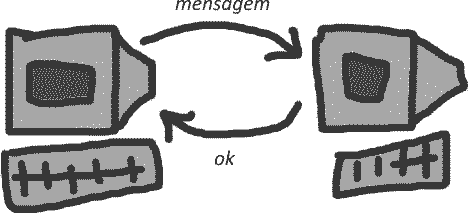
\includegraphics[width=0.9\linewidth]{unicast.png}%
				\caption{Unicast}%
				\label{fig:unicast}				
			\end{figure}	
		
			Caso seja necessário garantir o unicast, basta que o host remetente reenvie a mensagem até que ele receba a confirmação.
			Assim que ele receber a confirmação, simplesmente para de enviar a mensagem.
			O destinatário, ao identificar que recebeu a mensagem repetida, entende que o remetente não recebeu a confirmação e a reenvia somente uma vez.
			Quando o destinatário parar de receber reenvios da mensagem, ele compreende que o remetente finalmente recebeu a confirmação.
			
			É importante ressaltar que o destinatário não reenvia \msg{ok} por si só. 
			Ele só repete a confirmação quando recebe novamente a mensagem, assim, não é preciso que o destinatário confirme que recebeu a confirmação.
			
			\subsection{Medida de custo}
				Para se mensurar a quantidade de mensagens necessárias para a transmissão das mensagens nos sistemas de multicast, o unicast será a unidade de medida.
				
				Assim, o custo do unicast é 1 (é necessário 1 unicast confiável para entregar uma mensagem de um host para outro).
				Serão consideradas nessa unidade as mensagens de envio e as confirmações, bem como quaisquer retransmissões dessas que se fizerem necessárias.
				Portanto, o custo do unicast é 1.
				
				Para cada host, o custo do unicast $t_u$ é o mesmo do custo total $T_u$
				
				Será representado o custo em função dos $n$ hosts destinatários.
				No caso do unicast, por definição, esse número de destinatários $n = 1$ é fixo.
				Assim, 
				
				\begin{equation} \label{eq:unicast}					
					T_u(1) = t_u(1) = 1 					
				\end{equation}
			
				
		
		\section{Multicast}
		
			Para o multicast, utilizando comunicação ponto-a-ponto, é necessário elaborar uma estratégia um pouco mais complexa.
			A seguir, serão apresentados os dois protocolos propostos para envio de mensagens confiável de um para vários hosts.
		
		\section*{Propostas de protocolo}	
		
			\subsection{Multicast direto}
				A ideia mais direta e simples é que o host remetente envie para todos os destinatários como se fossem vários unicasts, enviando separadamente para todos.
				Para tornar esse multicast confiável basta fazer múltiplos unicasts confiáveis: para cada host que ainda não tenha confirmado recebimento, reenvia a mensagem.
				Quando for recebida a confirmação de um host, não é mais necessária retransmissão para ele. 
				A Figura~\ref{fig:multicast_direto} representa o multicast simples bem sucedido, realizado com vários unicasts isolados. 
			
				\begin{figure}[t]	%{R}{0.6\linewidth}%			
					\centering
					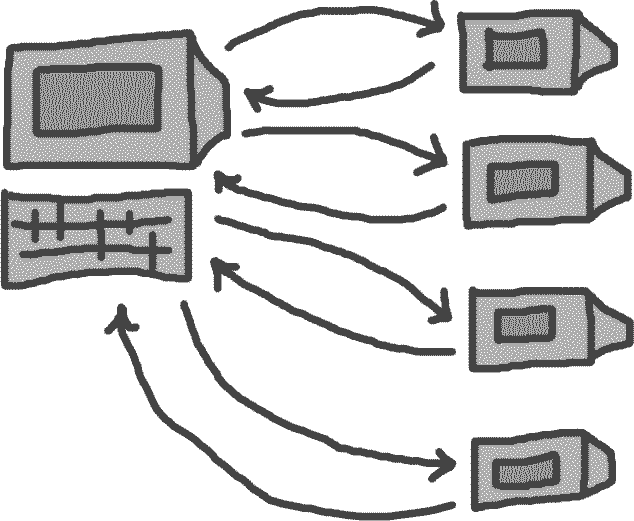
\includegraphics[width=0.9\linewidth]{multicast_simples.png}%
					\caption{Multicast direto}%
					\label{fig:multicast_direto}				
				\end{figure}
			
				\subsubsection{Falhas}			
			
					Caso não seja recebido confirmação de um host, como na Figura~\ref{fig:multicast_direto_falha}, o remetente compreende que houve falha nele.
					
					\begin{figure}[t]	%{R}{0.6\linewidth}%			
						\centering
						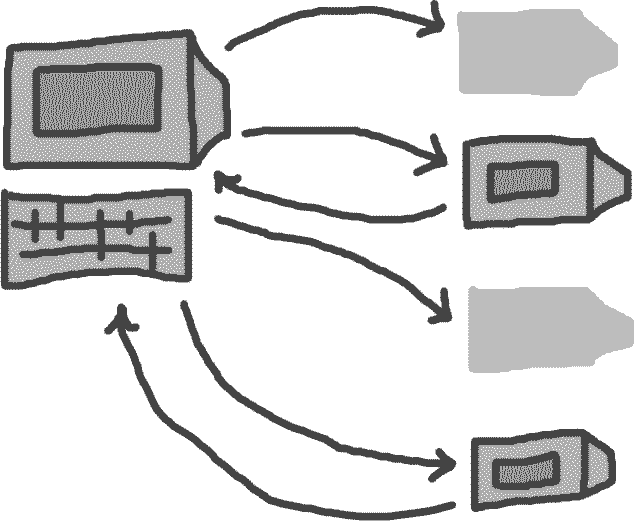
\includegraphics[width=0.9\linewidth]{multicast_simples_falha.png}%
						\caption{Multicast direto com falha}%
						\label{fig:multicast_direto_falha}				
					\end{figure}							
				
					Falsos positivos podem ocorrer quando não houver falha de fato do destinatário, mas suas confirmações não alcançarem o remetente.
					Falsos negativos podem ocorrer quando houver falha do destinatário depois dele enviar a confirmação (e dela ser recebida pelo remetente).
					
					Como os unicasts são isolados, a detecção de falha incorreta não levará a outros problemas na transmissão.
					
				\subsubsection{Custo}	
					Utilizando o unicast como unidade de medida, para $n$ hosts destinatários, o multicast direto custará $n$ unicasts no total.
					
					\begin{equation} \label{eq:multicast_direct}
						T_{m_D} (n) = n
					\end{equation}	
				
					Para os destinatários, o custo $t_{m_D}$ não passará de 1 (afinal, na perspectiva deles trata-se de um unicast).
					Porém, para o remetente o custo será igual ao total. 
					
					\begin{equation} \label{eq:multicast_direct_local}
						t_{m_D} (n) = n
					\end{equation}
			
			\subsection{Multicast em fileiras}
			
				Para reduzir o custo do multicast para o remetente, é possível distribuir os unicasts entre os hosts destinatários.
				Pode-se enviar a mensagem somente para um destinatário, informando-o de quais faltam receber.
				Este, então, envia a mensagem para o próximo, informando-o quais faltam, para que ele (e os demais) façam então o mesmo.
				No final, o último destinatário, informado de que mais ninguém precisa receber a mensagem além dele, envia para o remetente a confirmação de recebimento de todos os destinatários do grupo;
				
				Esse protocolo funciona como uma fileira: cada um pega uma cópia da mensagem e a repassa para o próximo. 
				A Figura~\ref{fig:multicast_fileira} mostra um exemplo sem falhas dessa transmissão.
				
				\begin{figure}[t]	%{R}{0.6\linewidth}%			
					\centering
					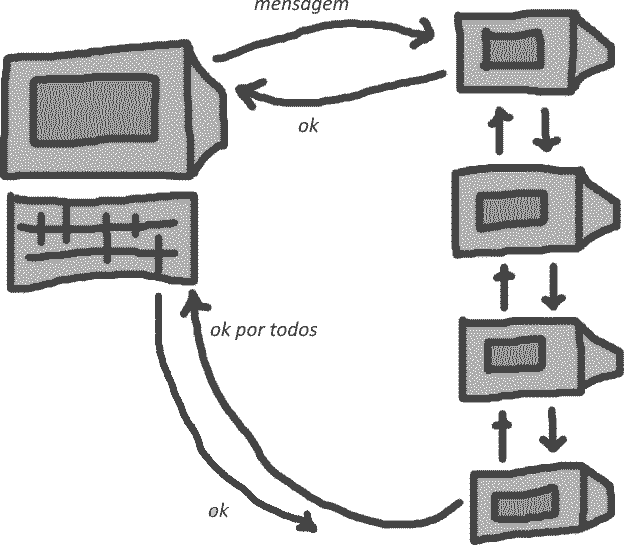
\includegraphics[width=0.9\linewidth]{multicast_encadeado.png}%
					\caption{Multicast em fileiras}%
					\label{fig:multicast_fileira}				
				\end{figure}														
			
				\subsubsection{Falhas} 	
				
					Caso não haja confirmação de recebimento em um dos unicasts (seja do remetente para o primeiro destinatário ou de um destinatário intermediário para o próximo), o host assume falha e envia para o destinatário seguinte (basicamente, envia para quem o host falho iria enviar depois).
					A Figura~\ref{fig:multicast_fileira_falha} ilustra os hosts enviando para os destinatários posteriores dos falhos.
					
					\begin{figure}[t]	%{R}{0.6\linewidth}%			
						\centering
						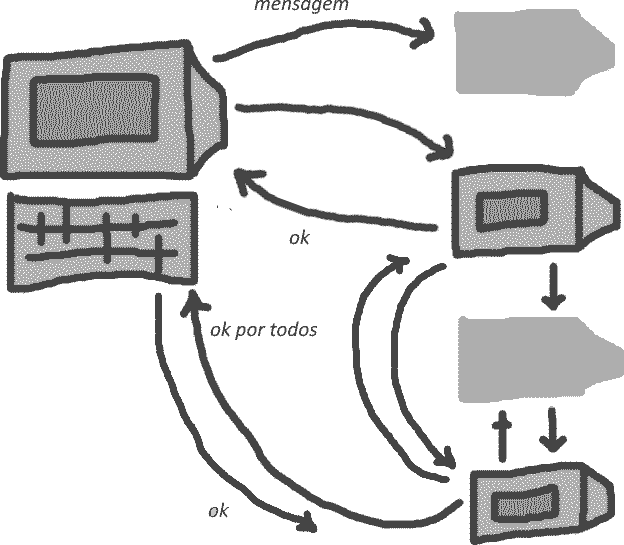
\includegraphics[width=0.9\linewidth]{multicast_encadeado_falha.png}%
						\caption{Multicast em fileiras com falhas em destinatários intermediários}%
						\label{fig:multicast_fileira_falha}				
					\end{figure}
				
					Quando o último destinatário tiver falha, o host que tiver timeout da confirmação dele irá assumir seu trabalho e responder para o remetente o total, como ilustrado pela Figura~\ref{fig:multicast_fileira_falha_final}. 
				
					\begin{figure}[t]	%{R}{0.6\linewidth}%			
						\centering
						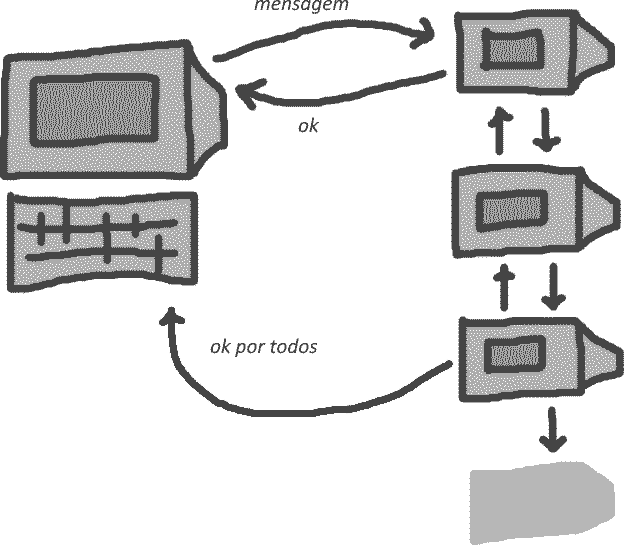
\includegraphics[width=0.9\linewidth]{multicast_encadeado_falha_final.png}%
						\caption{Multicast em fileiras com falha no último destinatário}%
						\label{fig:multicast_fileira_falha_final}				
					\end{figure}
					
					\subsubsection*{O problema da batata quente}
						Caso haja falha do destinatário depois de confirmar recebimento, mas antes de enviar a mensagem para o host seguinte, a responsabilidade de continuar a passagem da mensagem é perdida sem que o próximo host saiba.
						A sequência de transmissão seria interrompida silenciosamente e o remetente somente terá tido a confirmação do primeiro destinatário, achando que todos os demais falharam.
						
						A situação da batata quente perdida pode ser evitada se o host, após receber a confirmação que o próximo recebeu sua mensagem, mantenha a responsabilidade por um pouco mais de tempo (e gere um pouco mais de tráfego na rede).
						Ele pode enviar também para o host após o seu próximo (o mesmo para o qual esse próximo já confirmado estará enviando, caso não haja erro), evitando que o anel seja quebrado.
						
						Assim, como muitos problemas de sistemas distribuídos, a redundância aumenta a tolerância a falhas.
						Se o host enviar para os 2 próximos, ao invés só do próximo, um falso negativo por vez poderá ser remediado.
						Se enviar para os 3 próximos, 2 falsos negativos poderão ser remediados.
						Para os 4 próximos, 3 poderão e assim sucessivamente.
						
					\subsubsection*{Comprimento da fileira}
					
						Como esse protocolo cria uma estrutura de anel para envio sequencial, a volta completa nesse anel (a confirmação retornar para o remetente) pode demorar muito.
						Para evitar esse problema, pode-se criar subgrupos, enviando para várias fileiras menores.
						Limitando a quantidade de fileiras, a quantidade de unicasts por host não aumentará indefinidamente, como para o remetente do multicast direto.	
				
				\subsubsection{Custo}
				
					Considerando a versão básica (somente uma fileira, sem redundância), o envio de um host para o próximo usa $n$ unicasts, os quais se acrescenta 1, do último destinatário para o remetente.					
				
					\begin{equation} \label{eq:multicast_row}
						T_{m_R} (n) = n + 1
					\end{equation}	
				
					Embora o custo total e o tempo de envio sejam maiores que o multicast direto, nenhum host participa de mais do que 2 unicasts bem sucedidos, tornando $t_{m_R}$ mais igualitário.
					
					\begin{equation} \label{eq:multicast_row_local}
						t_{m_R} (n) = 2
					\end{equation}									
				
					Levando em consideração que a divisão do grupo de $n$ destinatários em até $k$ fileiras, o custo total será acrescido da quantidade de fileiras.	
					Os $r$ próximos hosts recebem mensagem de cada um multiplica esse custo.
					
					\begin{equation} \label{eq:multicast_row_safe}
						T_{m_R} (n) = (n + k)r
					\end{equation}
				
					O custo local também seria multiplicado pela redundância $r$, fazendo que, para os destinatários, $t_{m_R} (n) = 2r$.
					As $k$ fileiras separadas não influenciam nos custos locais dos hosts delas, mas aumentam o custo para o remetente.
			
					\begin{equation} \label{eq:multicast_row_safe_local}
						t_{m_R} (n) = 2kr
					\end{equation}
				
					É importante ressaltar que, mesmo que $k$ e $r$ aumentem (inclusive multiplicando) os custos do multicast, ambos são arbitrários e podem ser escolhidos para o cenário.
					Esses parâmetros não necessariamente aumentam com $n$, o que ainda permite escalabilidade sem sobrecarga do remetente.
					
	%\vfill				
					
	\section{Do programa}			
	
		A implementação foi feita em Python, exigindo esse ambiente para execução.
		Somente foram utilizadas bibliotecas nativas e o protocolo UDP para transmissão de pacotes. 
		Todas as funções e a classe de \texttt{multicast} estão definidas no arquivo \texttt{confia.py}
		
		\subsection{Inicialização}
		
			Para iniciar o programa é necessário fornecer argumentos.   	
			O único argumento obrigatório é o endereço de IP e a porta, no formato \texttt{<IP>:<Porta>}\footnote{\textbf{Exemplos}: \texttt{localhost:12345}, \texttt{127.0.0.1:65432} e \texttt{192.168.0.2:30500}}.
			A chamada básica seria \texttt{python3 confia.py -address <endereço>} mas, a depender da instalação, pode ser necessário chamar o Python com outros comandos, como \texttt{python} ou \texttt{py}.
			
			É possível nomear o host com a opção \texttt{-host <nome>}\footnote{Somente no arquivo em que houver um componente com o nome informado nos argumentos, o endereço poderá ser deduzido dali e omitido da chamada.} \\
			O atraso de resposta pode ser ajustado com \texttt{-delay <atraso>} e o período de heartbeat pode ser escolhido com \texttt{-heartbeat <período>}  \\
			O tempo máximo para confirmação (ou então detecção de falha) é escolhido com \texttt{-timeout <espera>} \\ 
			Todos os argumentos que representam intervalos de tempo são medidos em segundos e aceitam valores de ponto flutuante.
			
			A variação do multicast em fileiras, se desejada, pode ser feita com \texttt{-redundancy <redundância>} e \texttt{-max\_rows <fileiras>}
			
			Os argumentos que não forem entendidos como opções ou seus parâmetros serão tratados como nomes de arquivos com endereços e nomes dos componentes do grupo.
			Assim como na entrada pela linha de comando, os endereços devem estar no formato \texttt{<ip>:<porta>}
			
			Mais detalhes podem ser encontradas no arquivo \texttt{LEIAME.txt}
			
			
			
		\subsection{Utilização}	
		
			Os principais comandos do programa são: 
			\begin{enumerate}
				\item \texttt{help} exibe os métodos disponíveis
				
				\item \texttt{exit} sai do programa
				
				\item \texttt{direct} envia uma mensagem para todos os componentes do grupo e aguarda confirmações individuais de todos eles.
				A mensagem deve ser um literal válido para Python, como uma string, tupla, lista, um dicionário, inteiro ou ponto flutuante
				
				\item \texttt{row} envia uma mensagem para os primeiros componentes de cada fileira e aguarda confirmações de todas as fileiras.
				A mensagem deve ser um literal válido para Python, como uma string, tupla, lista, um dicionário, inteiro ou ponto flutuante
				
				\item \texttt{delay} altera o atraso para envio de mensagens
				
				\item \texttt{heartbeat} altera o período de tempo entre os heartbeats
				Caso seja 0, desativa o heartbeat permanentemente
				
				\item \texttt{pause}  pausa o heartbeat
				
				\item \texttt{resume}  retoma o heartbeat 
				
				\item \texttt{status}  mostra o último heartbeat de todos os componentes ativos conhecidos 
				
				\item \texttt{set\_max\_rows}  altera a quantidade máxima de fileiras para dividir o grupo no multicast em fileiras (row)
				
				\item \texttt{set\_redundancy}  altera a quantidade de cópias enviadas por fileira no multicast em fileiras (row)
				Essa quantidade é mesma que cada componente da fileira enviará para os próximos 								
				
			\end{enumerate}
			
				
	%\end{multicols}
\end{document}
